% This program is free software: you can redistribute it and/or modify
% it under the terms of the GNU AFFERO General Public License as published by
% the Free Software Foundation, either version 3 of the License, or
% (at your option) any later version.
% 
% This program is distributed in the hope that it will be useful,
% but WITHOUT ANY WARRANTY; without even the implied warranty of
% MERCHANTABILITY or FITNESS FOR A PARTICULAR PURPOSE.  See the
% GNU General Public License for more details.
% 
% You should have received a copy of the GNU AFFERO General Public License
% along with this program.  If not, see <https://www.gnu.org/licenses/>.
%
% Copyright (C) 2020 Mo Zhou <cdluminate@gmail.com>
%
\documentclass[9pt,twocolumn,times]{article}
\usepackage{times}
\usepackage[margin=0.9in]{geometry}
\usepackage{tikz}
\usepackage{pgflibraryshapes}
\usetikzlibrary{arrows.meta}
\usepackage{float}
\usepackage{amsmath}
\usepackage{amssymb}
\usepackage{graphicx}
\usepackage{xcolor}
\usepackage{hyperref}
\input{include/math_commands.tex}

\title{Computation Graph Cheat Sheet}
\author{Mo Zhou\\\small\texttt{<cdluminate@gmail.com>}}

\begin{document}

\maketitle
\tableofcontents

\section{Conventions}

Vectors are column vector by default.

\section{Automatic Differentiation}

\section{Atomic Modules}

\subsection{Level0: Scalar Ops}

\subsection{Level1: Vector-Vector Ops}

\subsection{Level2: Matrix-Vector Ops}

\begin{figure}[h]
	\centering
	\resizebox{0.618\columnwidth}{!}{%
		\input{tikz/cg-mv.tex}
	}
	\caption{GEMV: $\mW \vx = \vy$. (Linear)}
\end{figure}

	Forward Pass:
	\begin{equation}
		\mW_{(m\times k)} \cdot \vx_{(k)} = \vy_{(m)}
	\end{equation}

	Backward Pass:
	\begin{align}
		\frac{\partial L}{\partial\mW}_{(m\times k)} &=
		\frac{\partial L}{\partial\vy}_{(m)} \cdot \vx^T_{(1,k)}\\
		\frac{\partial L}{\partial\vx}_{(k)} &=
		\mW^T_{(k\times m)} \cdot \frac{\partial L}{\partial \vy}_{(m)}
	\end{align}

\subsection{Level3: Matrix-Matrix Ops}

\begin{figure}[h]
	\centering
	\resizebox{0.618\columnwidth}{!}{%
		% This program is free software: you can redistribute it and/or modify
% it under the terms of the GNU AFFERO General Public License as published by
% the Free Software Foundation, either version 3 of the License, or
% (at your option) any later version.
%
% This program is distributed in the hope that it will be useful,
% but WITHOUT ANY WARRANTY; without even the implied warranty of
% MERCHANTABILITY or FITNESS FOR A PARTICULAR PURPOSE.  See the
% GNU General Public License for more details.
%
% You should have received a copy of the GNU AFFERO General Public License
% along with this program.  If not, see <https://www.gnu.org/licenses/>.
%
% Copyright (C) 2020 Mo Zhou <cdluminate@gmail.com>
%
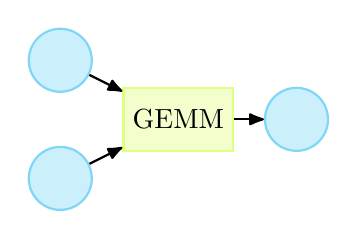
\begin{tikzpicture}[thick,minimum size=8mm]
	\node (w) at (0,0) [circle,draw=cyan!50,fill=cyan!20] {$\mW$};
	\node (x) at (0,-1.5) [circle,draw=cyan!50,fill=cyan!20] {$\mX$};
	\node (gemm) at (1.5,-0.75) [rectangle,draw=lime!50,fill=lime!20] {GEMM};
	\node (y) at (3,-0.75) [circle,draw=cyan!50,fill=cyan!20] {$\mY$};
	\draw [-{Latex[round]}] (w) -- (gemm);
	\draw [-{Latex[round]}] (x) -- (gemm);
	\draw [-{Latex[round]}] (gemm) -- (y);
\end{tikzpicture}

	}
	\caption{GEMM: $\mW \mX = \mY$. (Linear)}
\end{figure}

	Forward Pass:
	\begin{equation}
		\mW_{(m\times k)} \cdot \mX_{(k\times n)} = \mY_{(m\times n)}
	\end{equation}

	Backward Pass:
	\begin{align}
		\frac{\partial L}{\partial\mW}_{(m\times k)} &=
		\frac{\partial L}{\partial\mY}_{(m\times n)} \cdot \mX^T_{(n,k)}\\
		\frac{\partial L}{\partial\mX}_{(k\times n)} &=
		\mW^T_{(k\times m)} \cdot \frac{\partial L}{\partial \mY}_{(m\times n)}
	\end{align}

\subsection{Level4: Tensor Ops}

\section{Network Layers}

\end{document}
